\chapter{Process management}
\emph{Project management} is an horizontal activity lasting the entire development process. Project management is the task responsible of defining and controlling the effort needed, scheduling activities, estimating deliveries and organizing work and team allocation.

\begin{figure}[hbtp]
\centering
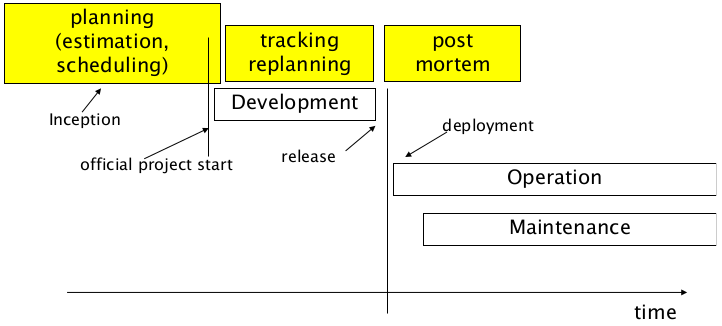
\includegraphics[scale=0.3]{images/process_management.png}
\caption{Process management}
\end{figure}

Projects do not start ``in zero time''. An inception phase is needed to analyze requirement, define an initial architecture, estimate duration and cost and perform a commercial proposal. When the proposal is signed, development can start.

\section{Concepts}
\paragraph{Resource}
Resources are both people and tools.

\paragraph{Activity}
An \emph{activity} requires time passed by resource to perform a defined and coherent task. A \emph{phase} is a set of activities.

\paragraph{Milestone}
A \emph{milestone} is key event or condition in the project with effects on subsequent activities, for instance a requirement document is a milestone because its acceptance by the customer leads to different activities in the process.

\paragraph{Deliverable}
A \emph{deliverable} is a product in the process, in a final or an intermediate state, internal or external, with contractual value or not.

\subsection{Techniques}
\paragraph{Gantt chart}
Gantt chart permits to plan a set of activities. Given the activities and temporal constraints among them, it provides an estimation of effort and timing.

\section{Measures}
\begin{itemize}
\item Process measures:
\begin{itemize}
\item Time, effort, cost;
\item Productivity;
\item Earned value;
\item Fault, failure, change.
\end{itemize}
\item Product measures:
\begin{itemize}
\item Functionality;
\item Size;
\item Price;
\item Modularity.
\end{itemize}
\end{itemize}

\paragraph{Calendar time or duration}
It can be measured in days, weeks, months on calendar. Relative duration from project start is typically used in planning, while absolute is typically used in controlling, remarking that transition from relative to actual is not 1 to 1.

\paragraph{Effort}
\emph{Effort} can be considered as time taken by staff to complete a task. It depends on calendar time and on people employed. It is measured in person hours and converted in cost.

\paragraph{Size}
\emph{Size} can regard different items.
\begin{itemize}
\item Source code (LOC);
\item Documents (number of pages, words, characters, figures or tables);
\item Test (number of test cases);
\item Entire project (function points).
\end{itemize}

\subparagraph{Line of codes}
It is needed to define what to count, e.g.,\@ comments, declarations, blank lines, what to include or exclude, e.g.,\@ libraries, external services, reused components and be aware that comparison between different languages are not meaningful.

\paragraph{Productivity}
Generally, \emph{productivity} is defined as output / effort, but in software defining output is difficult.

\subparagraph{LOC / effort}
\begin{itemize}
\item The lower level the language, the more productive the programmer. The same functionality takes more code to implement in a lower-level language than in a high-level language;
\item The more verbose the programmer, the higher the productivity. Measures of productivity based on lines of code suggest that programmers who write verbose code are more productive than programmers who write compact code.
\end{itemize}